%%%%%%%%%%%%%%%%%%%%%%%%%%%%%%%%%%%%%%%%%%%%%%%%%%%%%%%%%%%%%%%%%%%%%%%%%%%%%%%%%%
\begin{frame}[fragile]\frametitle{}
\begin{center}
{\Large Introduction}
\end{center}
\end{frame}



%%%%%%%%%%%%%%%%%%%%%%%%%%%%%%%%%%%%%%%%%%%%%%%%%%%%%%%%%%%
\begin{frame}[fragile]\frametitle{Intuition}

\begin{itemize}
\item Graph: Nodes connected by Edges
\item Knowledge Graph: Entities connected by Relations.
\end{itemize}
	  
\end{frame}




%%%%%%%%%%%%%%%%%%%%%%%%%%%%%%%%%%%%%%%%%%%%%%%%%%%%%%%%%%%%%%%%%%%%%%%%%%%%%%%%%%
\begin{frame}\frametitle{A Graph is}
{\emph \ldots a set of discrete objects, each of which has some set of relationships with the other objects}

Euler: Can we take a walk to all 4 islands, without crossing any of the bridge twice?

Abstraction (Does size of islands matter?):

\begin{center}
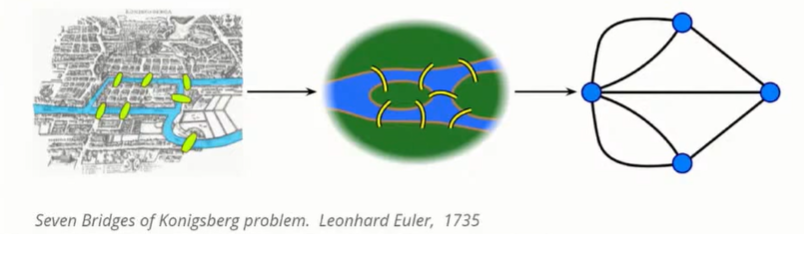
\includegraphics[width=\linewidth,keepaspectratio]{neo4j4}
\end{center}	  

Solution: No way!! What's the rule?

{\tiny (Ref: Introduction to Neo4j - a hands-on crash course - neo4j)}
\end{frame}


%%%%%%%%%%%%%%%%%%%%%%%%%%%%%%%%%%%%%%%%%%%%%%%%%%%%%%%%%%%
\begin{frame}[fragile]\frametitle{ Graph-structured Data Are Ubiquitous }

\begin{center}
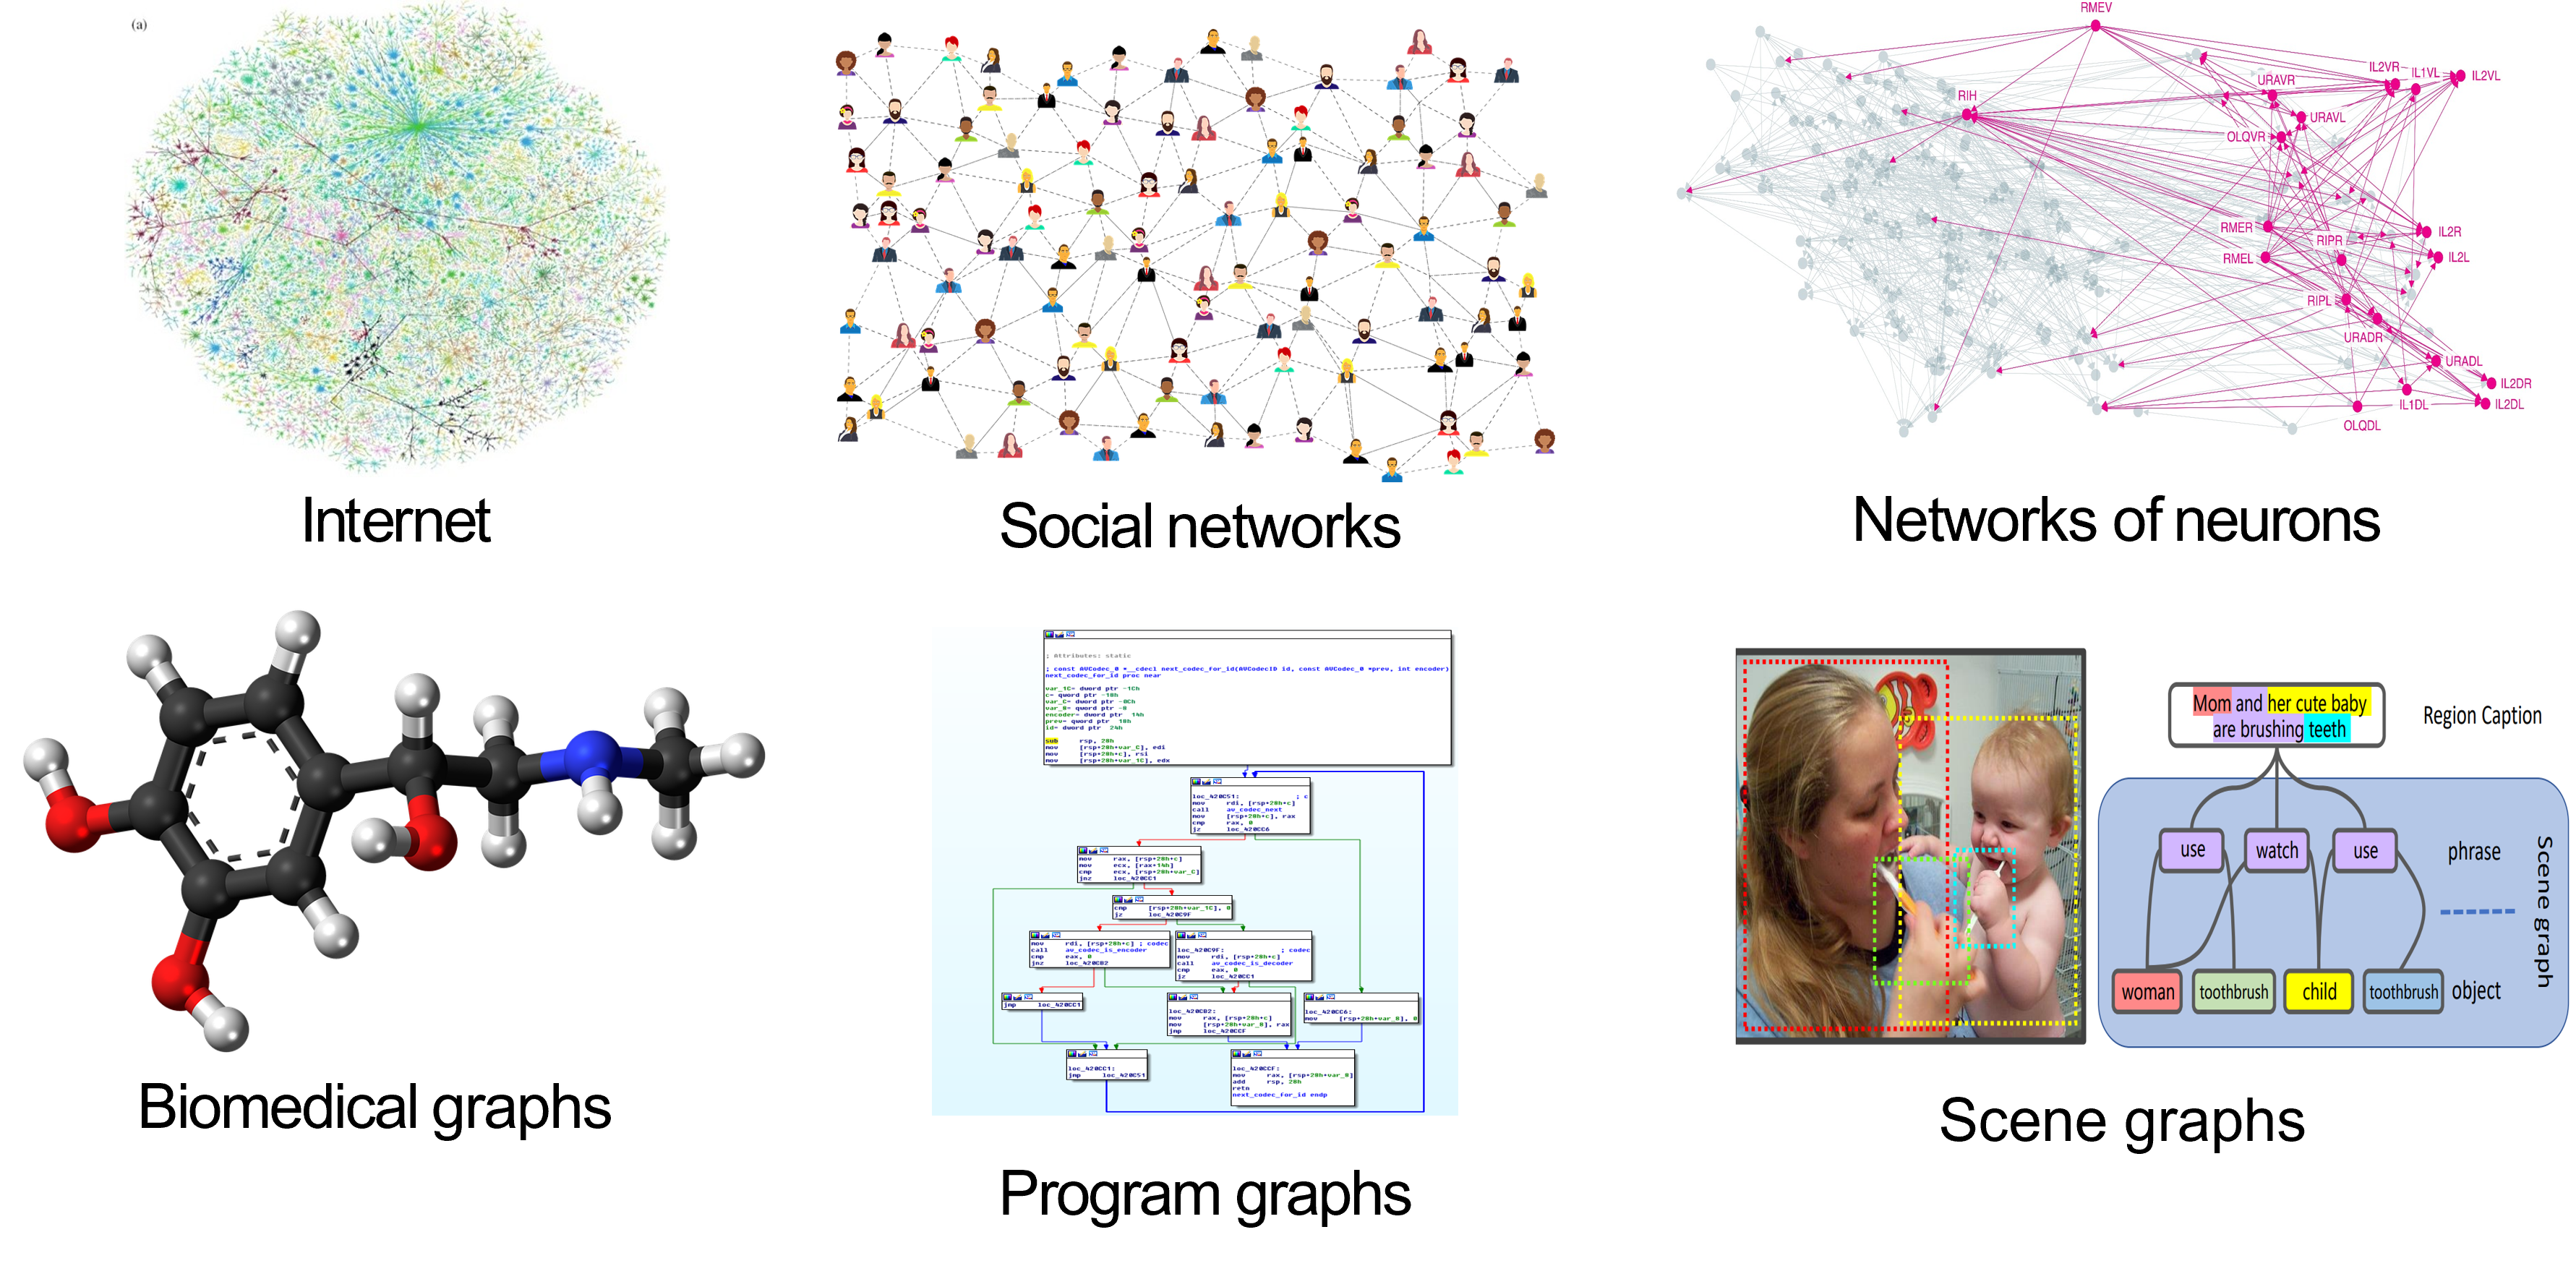
\includegraphics[width=\linewidth,keepaspectratio]{gnn1}
\end{center}	  

\end{frame}



%%%%%%%%%%%%%%%%%%%%%%%%%%%%%%%%%%%%%%%%%%%%%%%%%%%%%%%%%%%
\begin{frame}[fragile]\frametitle{Graphs: A Universal Language }

\begin{center}
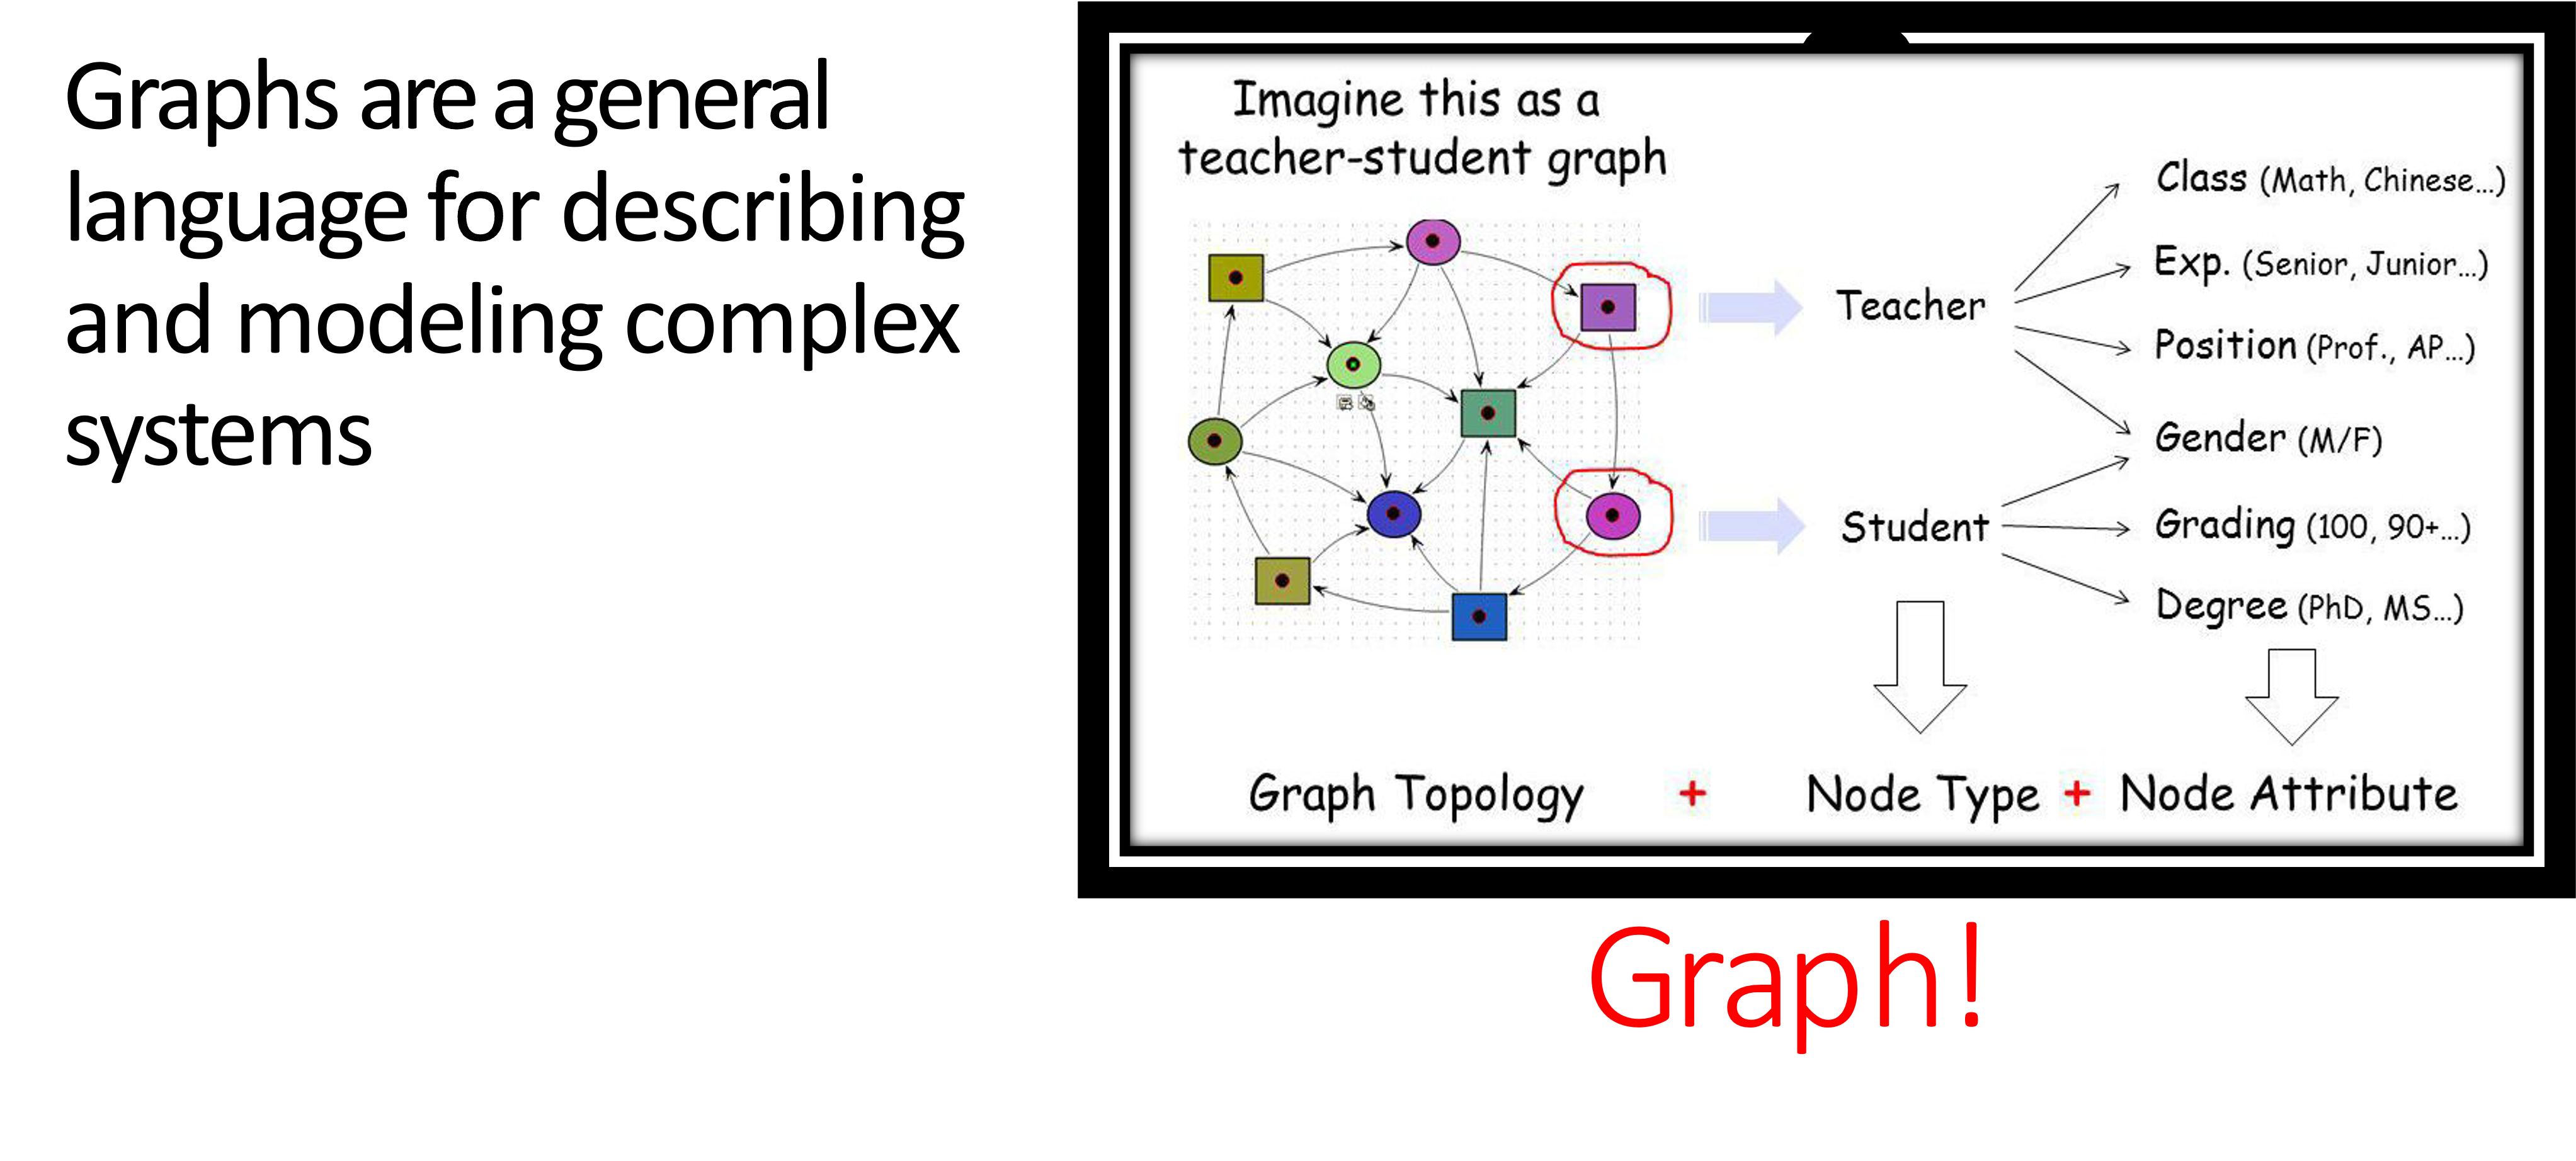
\includegraphics[width=\linewidth,keepaspectratio]{gnn4}
\end{center}	  

\end{frame}


%%%%%%%%%%%%%%%%%%%%%%%%%%%%%%%%%%%%%%%%%%%%%%%%%%%%%%%%%%%
\begin{frame}[fragile]\frametitle{Data as Graphs - Explicit }

\begin{center}
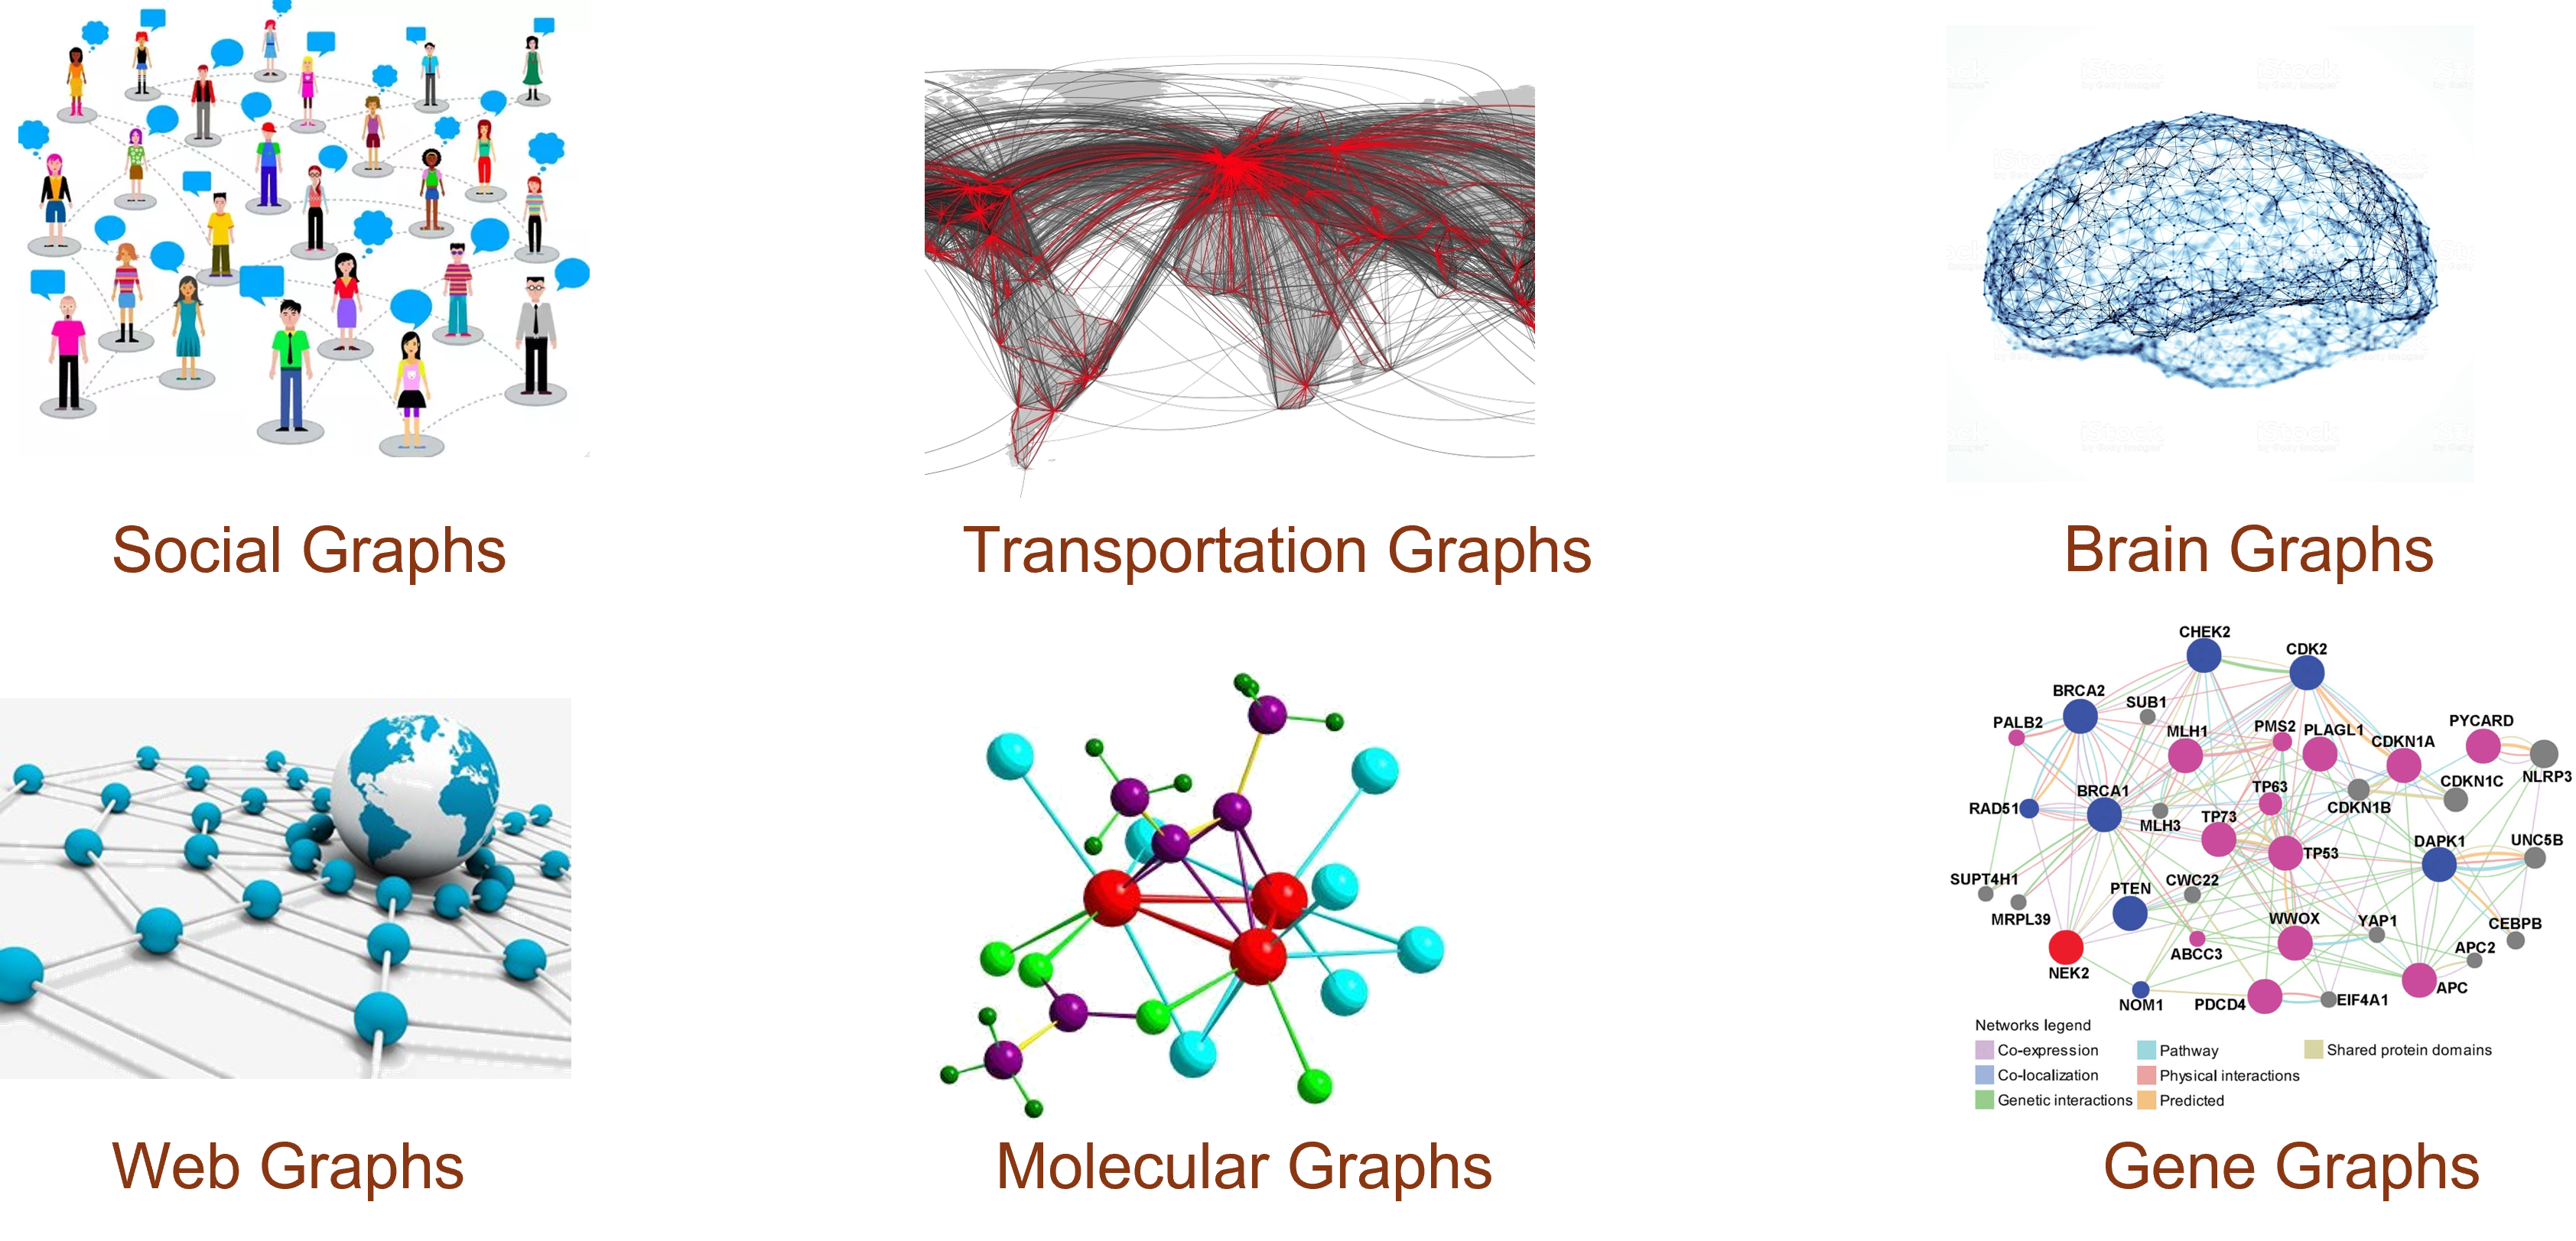
\includegraphics[width=\linewidth,keepaspectratio]{gnn5}
\end{center}	  

\end{frame}

%%%%%%%%%%%%%%%%%%%%%%%%%%%%%%%%%%%%%%%%%%%%%%%%%%%%%%%%%%%
\begin{frame}[fragile]\frametitle{Data as Graphs - Implicit }

\begin{center}
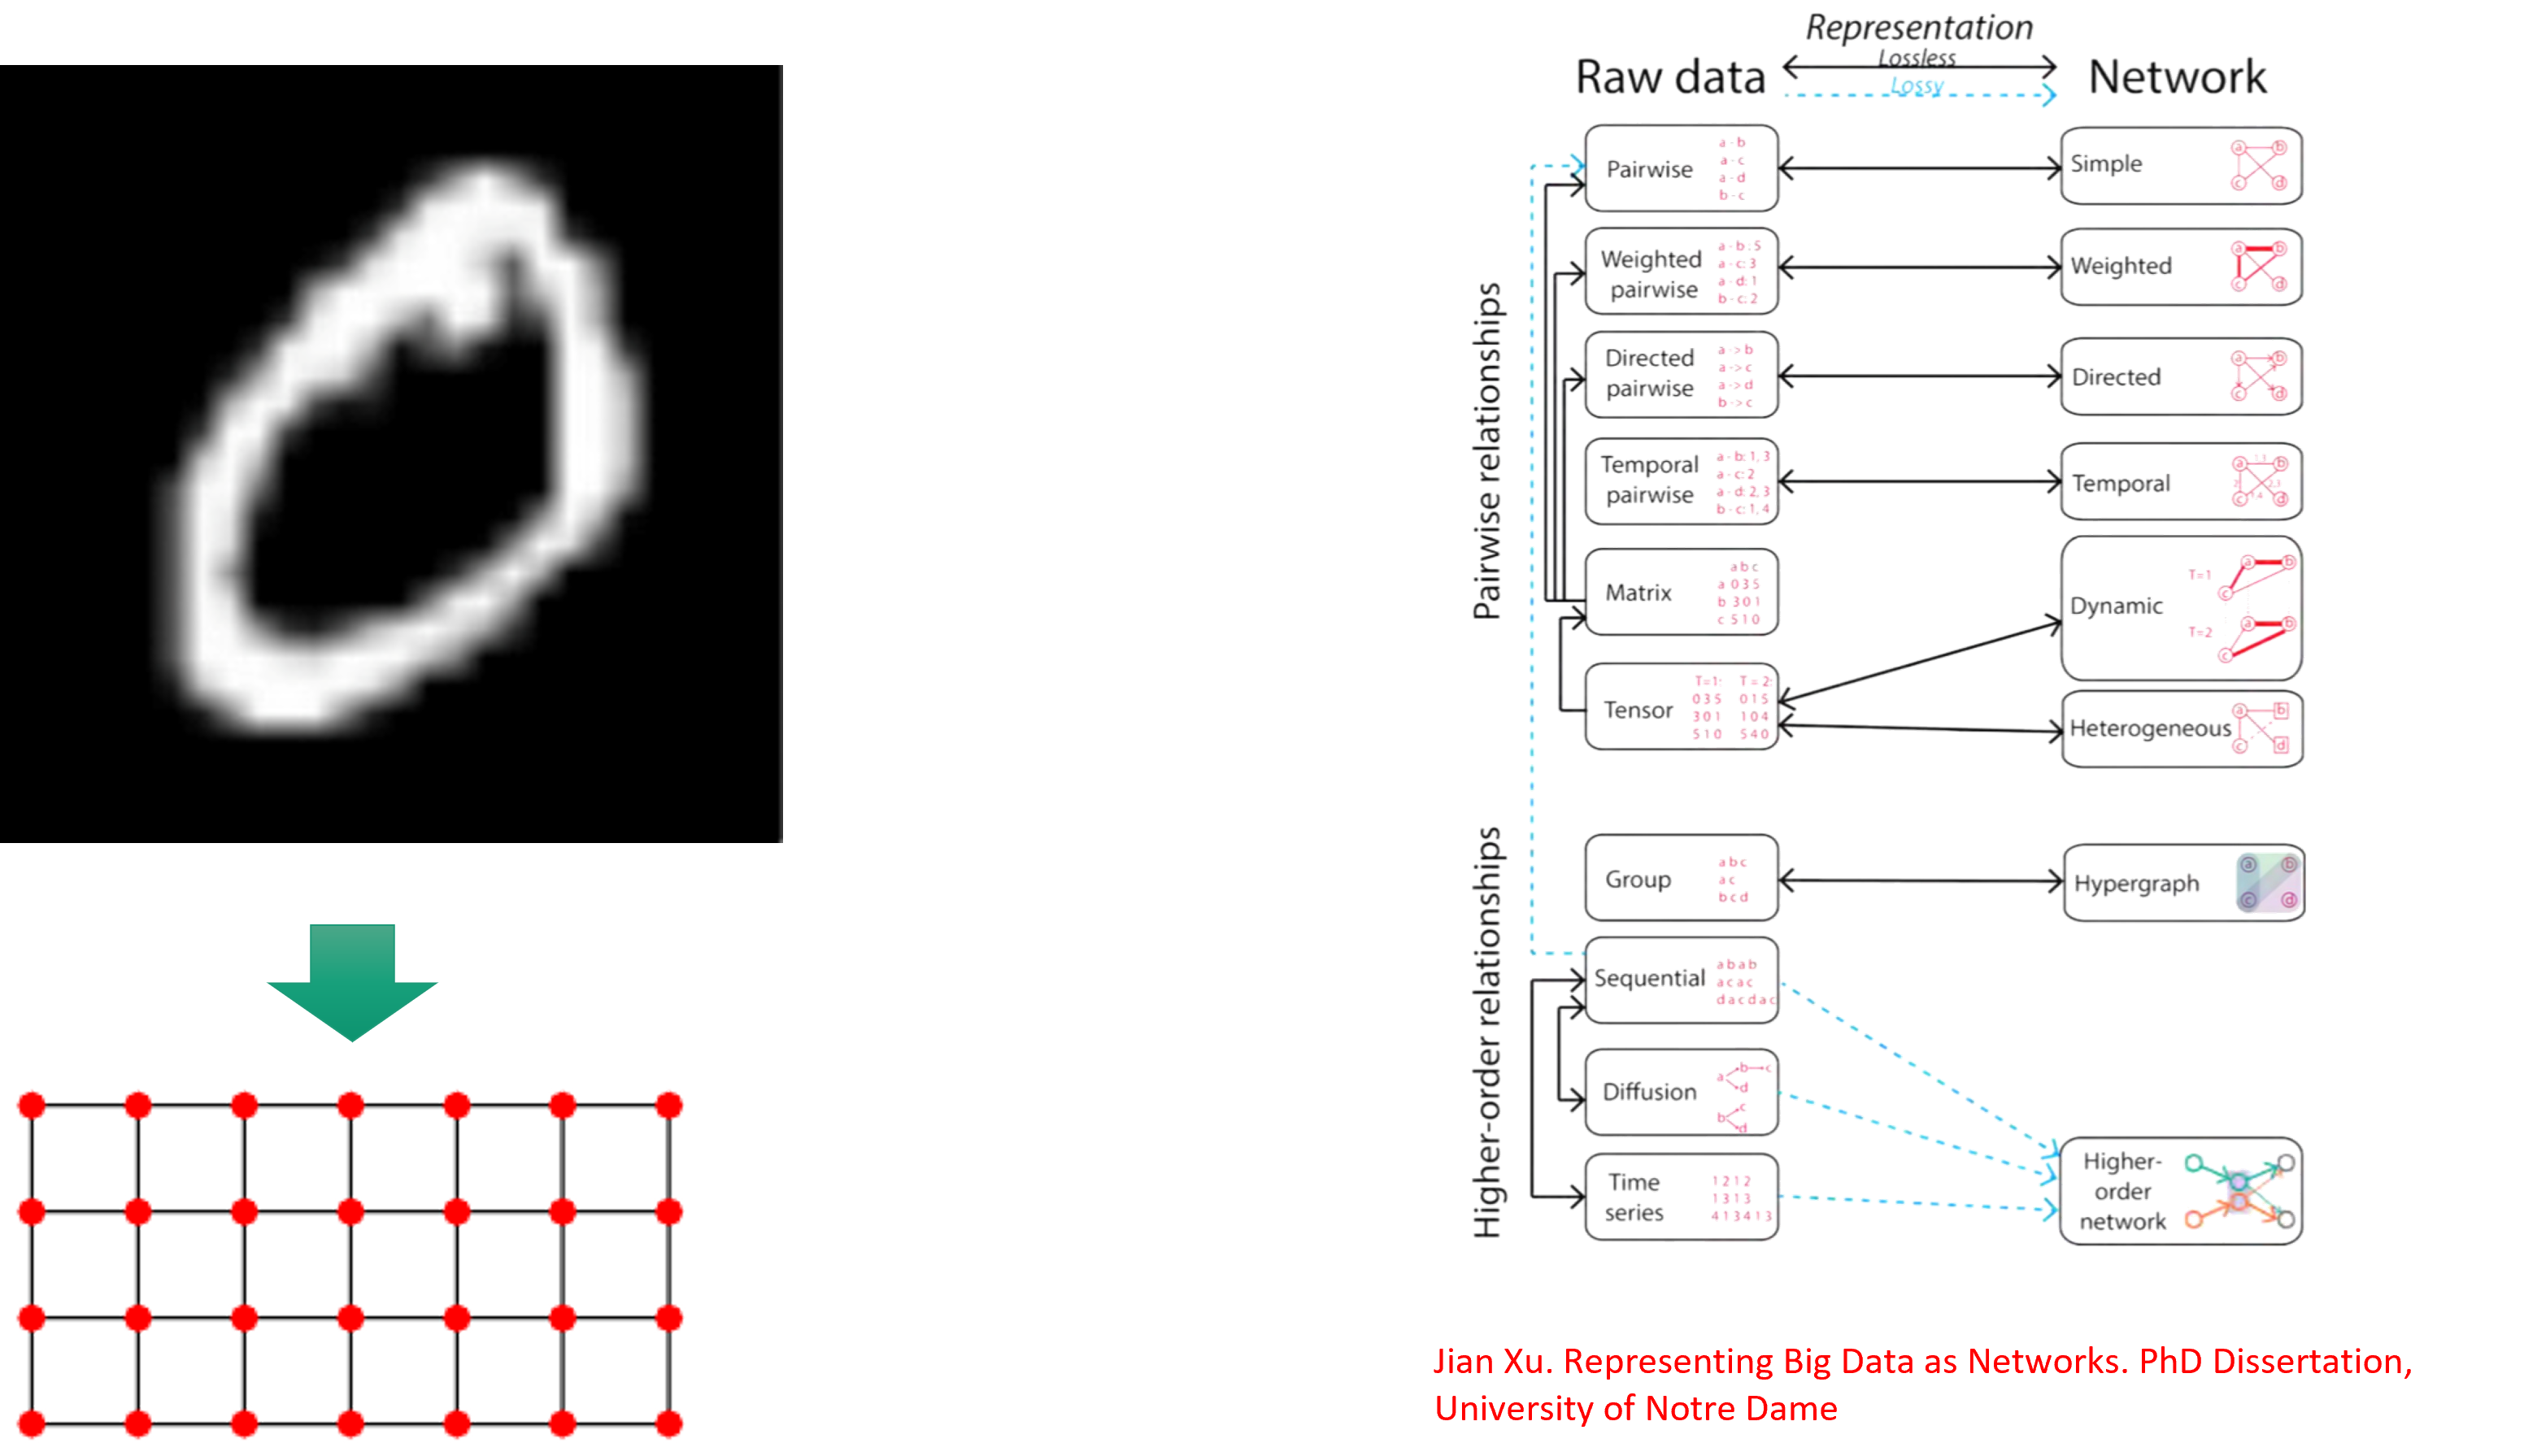
\includegraphics[width=\linewidth,keepaspectratio]{gnn6}
\end{center}	  

\end{frame}


%%%%%%%%%%%%%%%%%%%%%%%%%%%%%%%%%%%%%%%%%%%%%%%%%%%%%%%%%%%%%%%%%%%%%%%%%%%%%%%%%%
\begin{frame}\frametitle{ Graph Applications }

Across an organization, every department can benefit from graphs to answer questions 
like who or what is important, what should I do next, and what’s unusual about this?

\begin{center}
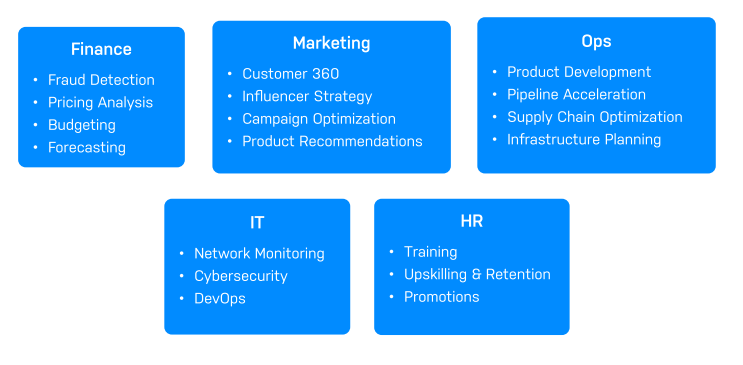
\includegraphics[width=\linewidth,keepaspectratio]{neo4j103}
\end{center}	  


{\tiny (Ref: 5 Graph Data Science Basics Everyone Should Know - neo4j)}
\end{frame}



%%%%%%%%%%%%%%%%%%%%%%%%%%%%%%%%%%%%%%%%%%%%%%%%%%%%%%%%%%%%%%%%%%%%%%%%%%%%%%%%%%
\begin{frame}\frametitle{A Knowledge Graph is}


\begin{columns}
    \begin{column}[T]{0.6\linewidth}

		Knowledge in Graph form.

			\begin{center}
			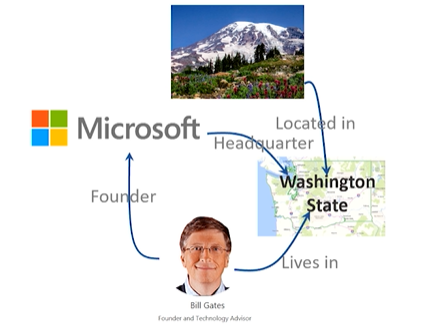
\includegraphics[width=\linewidth,keepaspectratio]{kg1}
			\end{center}	
    \end{column}
    \begin{column}[T]{0.4\linewidth}
			Embedded knowledge is:
			\begin{itemize}
			\item Microsoft is headquartered in Washington State.
			\item Bill Gates is a (co)Founder of Microsoft
			\item etc.
			\item Entities: Microsoft, Washington State, etc
			\item Relationships: founder, head, etc.
			\end{itemize}
    \end{column}
  \end{columns}
	

  

{\tiny (Ref: DAT278x - From Graph and Knowledge Graph - EdX course)}
\end{frame}

















%%%%%%%%%%%%%%%%%%%%%%%%%%%%%%%%%%%%%%%%%%%%%%%%%%%%%%%%%%%
\begin{frame}[fragile]\frametitle{References}

\begin{itemize}
\item DAT278x - From Graph and Knowledge Graph - EdX course
\end{itemize}
	  
\end{frame}
















%%%%%%%%%%%%%%%%%%%%%%%%%%%%%%%%%%%%%%%%%%%%%%%%%%%%%%%%%%%
\begin{frame}[fragile]\frametitle{Sample Picture Inclusion}

\begin{center}
\includegraphics[width=0.8\linewidth,keepaspectratio]{myphoto}
\end{center}	  
\end{frame}

%%%%%%%%%%%%%%%%%%%%%%%%%%%%%%%%%%%%%%%%%%%%%%%%%%%
\begin{frame}[fragile] \frametitle{Sample Code Listing}
\begin{lstlisting}
import aaa
\end{lstlisting}

\end{frame}

%%%%%%%%%%%%%%%%%%%%%%%%%%%%%%%%%%%%%%%%%%%%%%%%%%%%%%%%%%%
\begin{frame}[fragile]\frametitle{Sample Two Columns Slide}
\begin{columns}
    \begin{column}[T]{0.6\linewidth}
      \begin{itemize}
		\item aaa
	  \end{itemize}

    \end{column}
    \begin{column}[T]{0.4\linewidth}
      \begin{itemize}
		\item bbb
	  \end{itemize}
    \end{column}
  \end{columns}
\end{frame}

%%%%%%%%%%%%%%%%%%%%%%%%%%%%%%%%%%%%%%%%%%%%%%%%%%%%%%%%%%%%%%%%%%%%%%%%%%%%%%%%%%%
\begin{frame}[fragile]\frametitle{Sample Tabular Data}

aaa

\begin{tabular}{|c|c|}
	\hline
	Platform & Time (s) \\
	\hline \hline
	Python & $\sim$1500.0 \\
	\hline
	NumPy & 29.3 \\
	\hline
	Matlab & $\sim$29.0 \\
	\hline
	Octave & $\sim$60.0 \\
	\hline
	Blitz (C++) & 9.5 \\
	\hline
	Fortran & 2.5 \\
	\hline
	C & 2.2 \\
	\hline
\end{tabular}

\end{frame}
